\section{\textbf{Specifications}}

%\begin{figure}[h!]
%  \caption{Project Architecture}
%  \centering
%  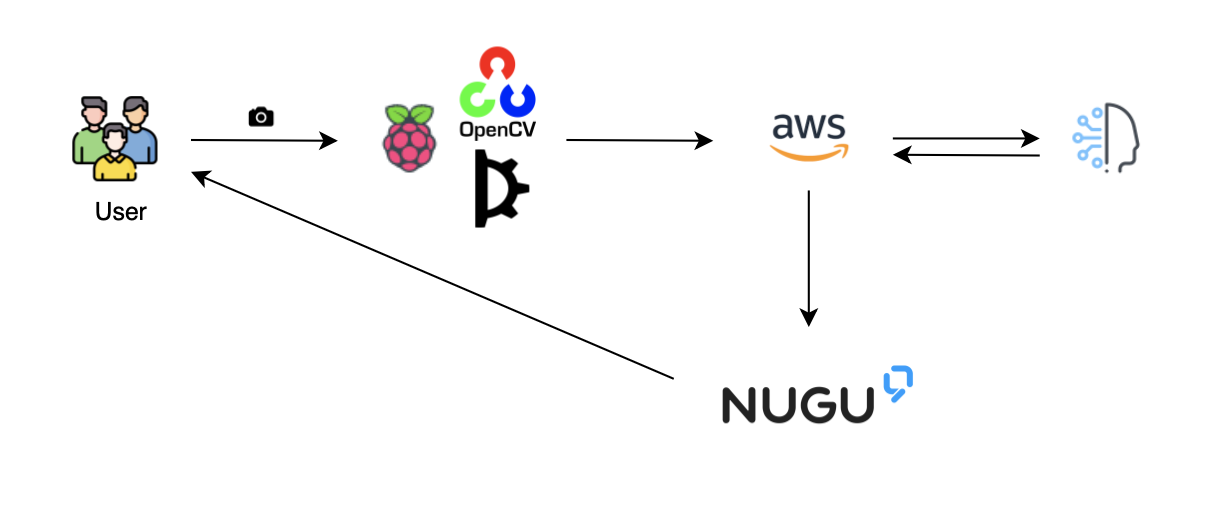
\includegraphics[width=0.5\textwidth]{images/SE-architecture.png}
%\end{figure}

\begin{figure}[h]
    \centering
    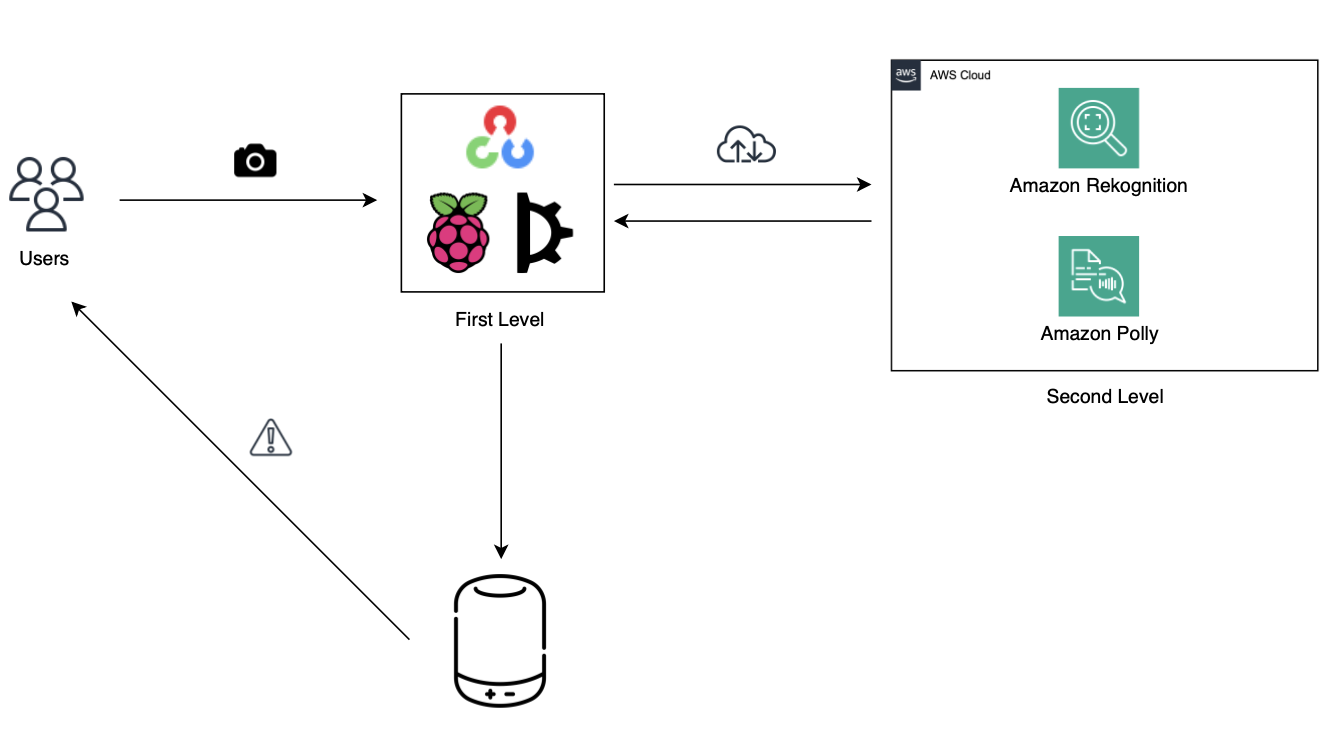
\includegraphics[width=1\linewidth]{images/architecture.png}
    \caption{Project Architecture}
    \label{fig:enter-label}
\end{figure}

\subsection{\textbf{Training AI model}}
% 인공지능 모델을 데이터를 기반으로 학습시키는 과정이다. 데이터는 kaggle의 'Face Images of Acute Stroke and Non Acute Stroke' 의 38MB 가량 이미지이다. Stroke face 이미지 약 1,600장, non stroke face 약 2,400장으로 총 4,000여장의 데이터로 학습을 진행한다. 학습 과정에서 이미지 전처리는 다음과 같이 진행한다. (200x2000x3)의 tensor로 변환하고 flatten 한다. label은 stroke face를 1, non-stroke face를 0으로 표기했고 SVM과 Transformer 모델을 위와 같은 조건에서 Google Colab에서 학습시킨다.
This is the process of learning an artificial intelligence model based on data. The data is a 38MB image from kaggle's 'Face Images of Acute Stroke and Non Acute Stroke'. Training is conducted with a total of 4,000 pieces of data, including about 1,600 stroke face images and 2,400 non-stroke face images. Image preprocessing during the learning process proceeds as follows. Convert to a tensor of (200x200x3) and flatten. The label indicates the stroke face as 1 and the non-stroke face as 0, and the SVM and Transformer models are trained in Google Colab under the above conditions.\\

\subsubsection{\textbf{Support Vector Machine}}
% Support Vector Machine을 사용하기 위해서 scikit-learn에서 svm 라이브러리를 import한다. 설정할 수 있는 hyper parameter는 다음과 같다.
\begin{itemize}
    \item C(Regularization Parameter): C is a parameter that controls the penalty for misclassifications. A small C value sets a low penalty for misclassifications, making the model fit the training data more. A large C value sets a high penalty for misclassifications, encouraging the model to achieve higher accuracy on the training data. The appropriate value for C is determined through cross-validation.
    \item Kernel: SVM supports various kernel functions. The most commonly used kernels include the linear kernel, polynomial kernel, and Radial Basis Function (RBF) kernel. The choice of kernel depends on the data's characteristics and the problem at hand.
    \item Gamma: When using the RBF kernel, Gamma controls the flexibility of the decision boundary. A small Gamma value makes the decision boundary smoother, while a large Gamma value makes the decision boundary more complex. The appropriate value for Gamma is also determined through cross-validation.
\end{itemize}
% 이런 다양한 hyper parameter 중 kernel은 rbf kernel을 사용하고 나머지 두 파라미터를 sklearn 라이브러리의 GridSearchCV method를 사용해 최적의 값을 구한다.

\subsubsection{\textbf{ViT}}
\cite{vision-transformers-medium}
% ViT는 다양한 모듈이 모여 구성된다. 모듈은 다음과 같이 구성된다.
ViT is composed of various modules. The module is composed as follows.\\

\textbf{Patchify} \\
The transformer encoder was developed with sequence data in mind, such as English sentences. However, an image is not a sequence. So we have to “sequencify” an image. We break it into multiple sub-images and map each sub-image to a vector.

We do so by simply reshaping our input, which has size (N, C, H, W), to size (N, \#Patches, Patch dimensionality), where the dimensionality of a patch is adjusted accordingly.\\

\textbf{Adding classification tokens} \\
If you look closely at the architecture picture, you will notice that also a “v\_class” token is passed to the Transformer Encoder.

Simply put, this is a special token that we add to our model that has the role of capturing information about the other tokens. This will happen with the MSA block (later on). When information about all other tokens will be present here, we will be able to classify the image using only this special token. The initial value of the special token (the one fed to the transformer encoder) is a parameter of the model that needs to be learned.

If we wanted to do another downstream task, we would just need to add another special token for the other downstream task (for example, classifying a digit as higher than 5 or lower) and a classifier that takes as input this new token.\\

\textbf{Positional Encoding} \\
As anticipated, positional encoding allows the model to understand where each patch would be placed in the original image. While it is theoretically possible to learn such positional embeddings, previous work by Vaswani et. al. suggests that we can just add sines and cosines waves.

In particular, positional encoding adds high-frequency values to the first dimensions and low-frequency values to the latter dimensions.

In each sequence, for token i we add to its j-th coordinate the following value:


\[p_{i, j} = \left\{\begin{matrix}
sin\left(\frac{i}{10000^{\frac{j}{d_{emb\_dim}}}}\right) \\ cos\left(\frac{i}{10000^{\frac{j}{d_{emb\_dim}}}}\right)
\end{matrix}\right.\]

This positional embedding is a function of the number of elements in the sequence and the dimensionality of each element. Thus, it is always a 2-dimensional tensor or “rectangle”.

Here’s a simple function that, given the number of tokens and the dimensionality of each of them, outputs a matrix where each coordinate (i,j) is the value to be added to token i in dimension j.\\

\textbf{Layer Normalization}
Layer normalization is a popular block that, given an input, subtracts its mean and divides by the standard deviation.

However, we commonly apply layer normalization to an (N, d) input, where d is the dimensionality. Luckily, also the Layer Normalization module generalizes to multiple dimensions.

Layer normalization is applied to the last dimension only. We can thus make each of our 50x8 matrices (representing a single sequence) have mean 0 and std 1.\\

\textbf{Multi-head Self Attention} \\
Simply put: we want, for a single image, each patch to get updated based on some similarity measure with the other patches. We do so by linearly mapping each patch to 3 distinct vectors: \(\mathbf{q}, \mathbf{k}\), and \(\mathbf{v}\) (query, key, value).


Then, for a single patch, we are going to compute the dot product between its q vector with all of the k vectors, divide by the square root of the dimensionality of these vectors, softmax these so-called attention cues, and finally multiply each attention cue with the v vectors associated with the different k vectors and sum all up.

In this way, each patch assumes a new value that is based on its similarity (after the linear mapping to \(\mathbf{q}, \mathbf{k}\) and \(\mathbf{v}\)) with other patches. This whole procedure, however, is carried out H times on H sub-vectors of our current 8-dimensional patches, where H is the number of Heads. If you’re unfamiliar with the attention and multi-head attention mechanisms, I suggest you read this nice post by Yasuto Tamura.

Once all results are obtained, they are concatenated together. Finally, the result is passed through a linear layer (for good measure).

The intuitive idea behind attention is that it allows modeling the relationship between the inputs. What makes a ‘0’ a zero are not the individual pixel values, but how they relate to each other.\\

\textbf{Residual Connection} \\
A residual connection consists in just adding the original input to the result of some computation. This, intuitively, allows a network to become more powerful while also preserving the set of possible functions that the model can approximate.

With this self-attention mechanism, the class token (first token of each of the N sequences) now has information regarding all other tokens.\\

\textbf{Classfication MLP} \\
Finally, we can extract just the classification token (first token) out of our N sequences, and use each token to get N classifications.



\\
\subsection{\textbf{Saving trained AI model}}
% 학습이 완료된 인공지능 모델을 파일로 저장해 웹 서버에 배포할 수 있도록 저장한다. 저장하는 형식은 여러가지가 있다. 우리가 사용한 방식은 joblib이다. joblib은 dump(), load() 명령어로 단순하게 모델을 저장하고 불러올 수 있기 때문에 선택했다. Google Colab에서 학습이 완료된 인공지능 모델을 joblib.dump() 명령으로 Google Drive에 저장하고 local computer로 다운로드한다.
The trained artificial intelligence model is saved as a file so that it can be distributed to a web server. There are various saving formats. The method we used is joblib. joblib was chosen because it allows you to simply save and load models with the dump() and load() commands. Save the artificial intelligence model that has completed training in Google Colab to Google Drive using the joblib.dump() command and download it to your local computer.\\

\subsection{\textbf{Loading trained AI model}}
% 저장한 방식과 같이 joblib 라이브러리를 사용해서 학습이 완료된 인공지능 모델을 파일에서부터 불러올 수 있다. Google Colab에서 인공지능을 학습시키고 저장된 모델을 AWS Lightsail에 scp 명령어를 통해 local에서 옮긴다. 이로써 모델을 AWS Lightsail 가상 머신으로 웹 서버를 이용해 배포할 준비를 마친다.
Just like how you saved it, you can load the trained artificial intelligence model from a file using the joblib library. Train artificial intelligence in Google Colab and move the saved model locally to AWS Lightsail using the scp command. This completes the preparation to deploy the model as an AWS Lightsail virtual machine using a web server.\\

\subsection{\textbf{Classifying Image with trained AI model}}
% 인공지능 모델을 학습시킬 때와 유사하게 이미지를 전처리한다. (200x200x3) tensor로 이미지를 변환한다. skimage 라이브러리의 resize 함수를 호출해 처리한다. 이후 flatten 시켜 이미지 전처리를 완료한다. load 된 인공지능 모델로 predict 메소드를 호출하고 전처리된 이미지를 파라미터로 넘겨줘서 예측값을 반환하도록 한다. 이때, 단순히 0 또는 1의 classification 된 결과뿐만 아니라 각 확률값을 같이 반환하도록 해서 판단의 근거를 사용자에게도 알려준다.
Images are preprocessed similarly to when training an artificial intelligence model. Convert the image to (200x200x3) tensor. Process it by calling the resize function of the 'skimage' library. Afterwards, image preprocessing is completed by flattening. Call the predict method with the loaded artificial intelligence model and return the predicted value by passing the preprocessed image as a parameter. At this time, not only the classified result of 0 or 1 is returned, but also the probability value is returned to inform the user of the basis for the judgment.\\

\subsection{\textbf{Returning the result}}
% 반환된 값을 다시 웹 통신으로 라즈베리 파이로 전송해야 하기 때문에 JSON 객체로 변경한다. 총 3개의 key-value 값으로 이루어져 있다. key는 다음과 같다. 'prediction', 'probability_0', 'probability_1'로 각각 예측값, non-Stroke 확률, Stroke 확률을 나타낸다. 예시 객체는 다음과 같다.
Because the returned value needs to be sent back to the Raspberry Pi via web communication, it is changed to a JSON object. It consists of a total of three key-value values. The key is as follows. 'prediction', 'probability\_0', and 'probability\_1' represent the predicted value, non-stroke probability, and stroke probability, respectively. Example objects are as follows:
\begin{verbatim}
{
    'prediction': result_list[0],
    'probability_0': probability[0][0],
    'probability_1': probability[0][1]
}
\end{verbatim}
\\

\subsection{\textbf{Get Image with API}}
% FastAPI의 File, UploadFile 라이브러리를 이용하면 웹 서버를 통해 전송된 사진을 프로그램 내에서 처리할 수 있다. skimage.io 라이브러리의 imread 메소드와 결합하여 사용하면 training 과정에서와 같은 로직으로 이미지를 인공지능 모델에 전달할 수 있다. 예시 코드는 다음과 같다.
Using FastAPI's File and UploadFile libraries, images sent through a web server can be processed within the program. When used in combination with the 'imread' method of the skimage.io library, images can be transmitted to the artificial intelligence model using the same logic as in the training process. Example code is as follows:
\begin{verbatim}
{
    img_array = imread(file.file)
}
\end{verbatim}
\\
\subsection{\textbf{Post the result with API}}
% 위의 Returning the result에서 Json format으로 예측값을 변환하여 만든 값을 다시 라즈베리 파이로 보내준다. @app.post("/classify/") annotation이 붙어있는 함수에서 return을 하게 되면 해당 이미지 파일을 보내준 곳으로 응답을 보내기 때문에 classification을 하는 함수 위에 해당 annotation을 붙이고 위의 Json format을 return 하면 Post할 수 있다.
In 'Returning the result' above, the predicted value is converted to JSON format and the resulting value is sent back to the Raspberry Pi. When you return from a function with the @app.post("/classify/") annotation, a response is sent to the place where the image file was sent, so if you attach the annotation to the function that performs classification and return the above Json format, you can Post.\\

\subsection{\textbf{Encapsulate the AI model}}
% 위에서 언급한 모든 내용을 한 파일로 구현할 수 있다. app.py 파일을 제작하고 이미지 전처리, 인공지능 모델에서의 prediction, return값을 제작하고 이 함수 위에 annotation을 붙여 모든 일을 한번에 처리하도록 encapsulation 할 수 있다.
Everything mentioned above can be implemented in one file. You can create an app.py file, create image preprocessing, prediction from an artificial intelligence model, and return value, and attach an annotation on top of this function to encapsulate it so that all tasks are processed at once.\\

\subsection{\textbf{Run the Web Server}}
% Uvicorn 으로 app.py 파일을 실행할 수 있다. 이 때, 외부 IP도 접속 가능하도록 아래와 같이 추가 명령어를 기입해 실행한다.
You can run the app.py file with Uvicorn. At this time, enter and execute the additional command as shown below to enable connection to the external IP.
\begin{verbatim}
    uvicorn app:app --reload --host=0.0.0.0
\end{verbatim}


\subsection{\textbf{Amazon Rekognition}}
\subsubsection{\textbf{Preparing Data}}
% 학습에 필요한 데이터는 이전과 동일하게 stoke data 1200개 가량, no_stroke data 2500개 가량으로 총 3700 여개로 구성되었다. Amazon Rekogniton에서는 데이터가 속한 폴더의 이름을 이미지의 레이블로 자동으로 설정할 수 있다. 이 기능을 이용해 편리하게 데이터의 라벨링을 완료했고 학습용 데이터와 테스트용 데이터를 8:2의 비율로 나누었다. 따로 이미지의 색을 흑백으로 바꾸거나 이미지의 사이즈를 통일시키는 작업은 처리하지 않았다.
The data needed for learning was the same as before, consisting of approximately 1,200 stroke data and 2,500 no\_stroke data, for a total of 3,700 pieces. Amazon Rekogniton can automatically set the name of the folder containing the data as the label of the image. Using this function, we conveniently completed labeling the data and divided the training data and testing data in a ratio of 8:2. No work was done to change the color of the image to black and white or to unify the size of the image.

\begin{figure}[h]
    \centering
    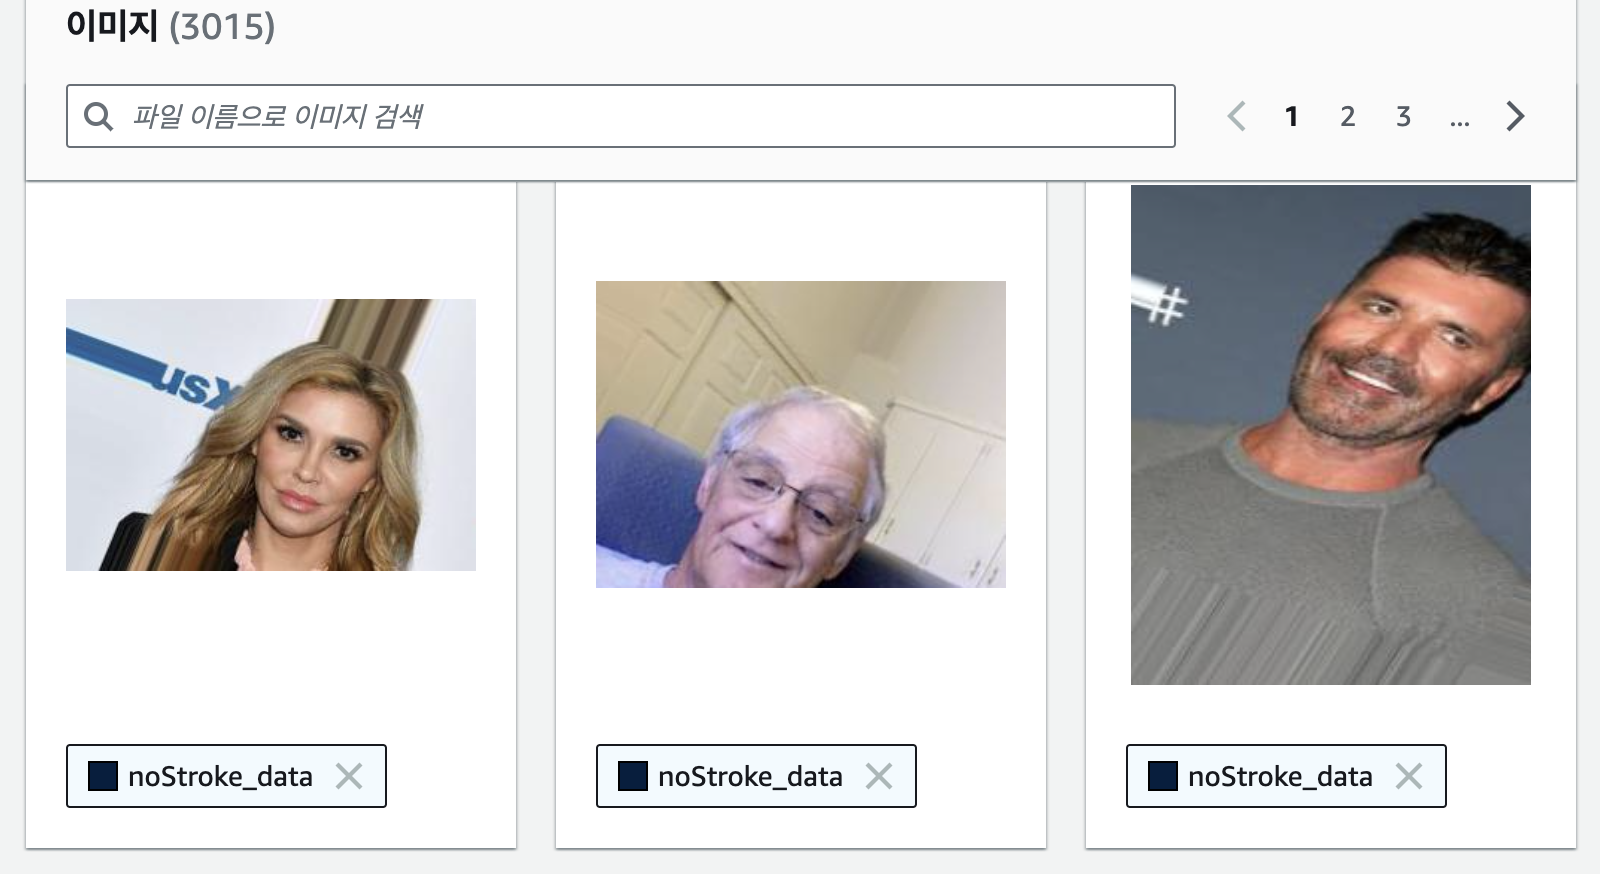
\includegraphics[width=8.5cm]{images/rek_data.png}
    \caption{Dataset for training Amazon Rekognition}
\end{figure}


\subsubsection{\textbf{Training Rekognition model}}
% 위에서 준비한 데이터로 Amazon Rekognition 모델을 학습시킨다. 하이퍼파라미터나 추가적으로 설정해야하는 것들은 자동으로 설정하고 그 중에서 최적의 파라미터를 자동으로 찾아주기 때문에 optimizer나 파라미터를 설정하지 않고 바로 모델 훈련을 진행했다.
Train the Amazon Rekognition model with the data prepared above. Hyperparameters and those that need to be set additionally are automatically set and the optimal parameters are automatically found, so model training was performed immediately without setting the optimizer or parameters.


\begin{figure}[h]
    \centering
    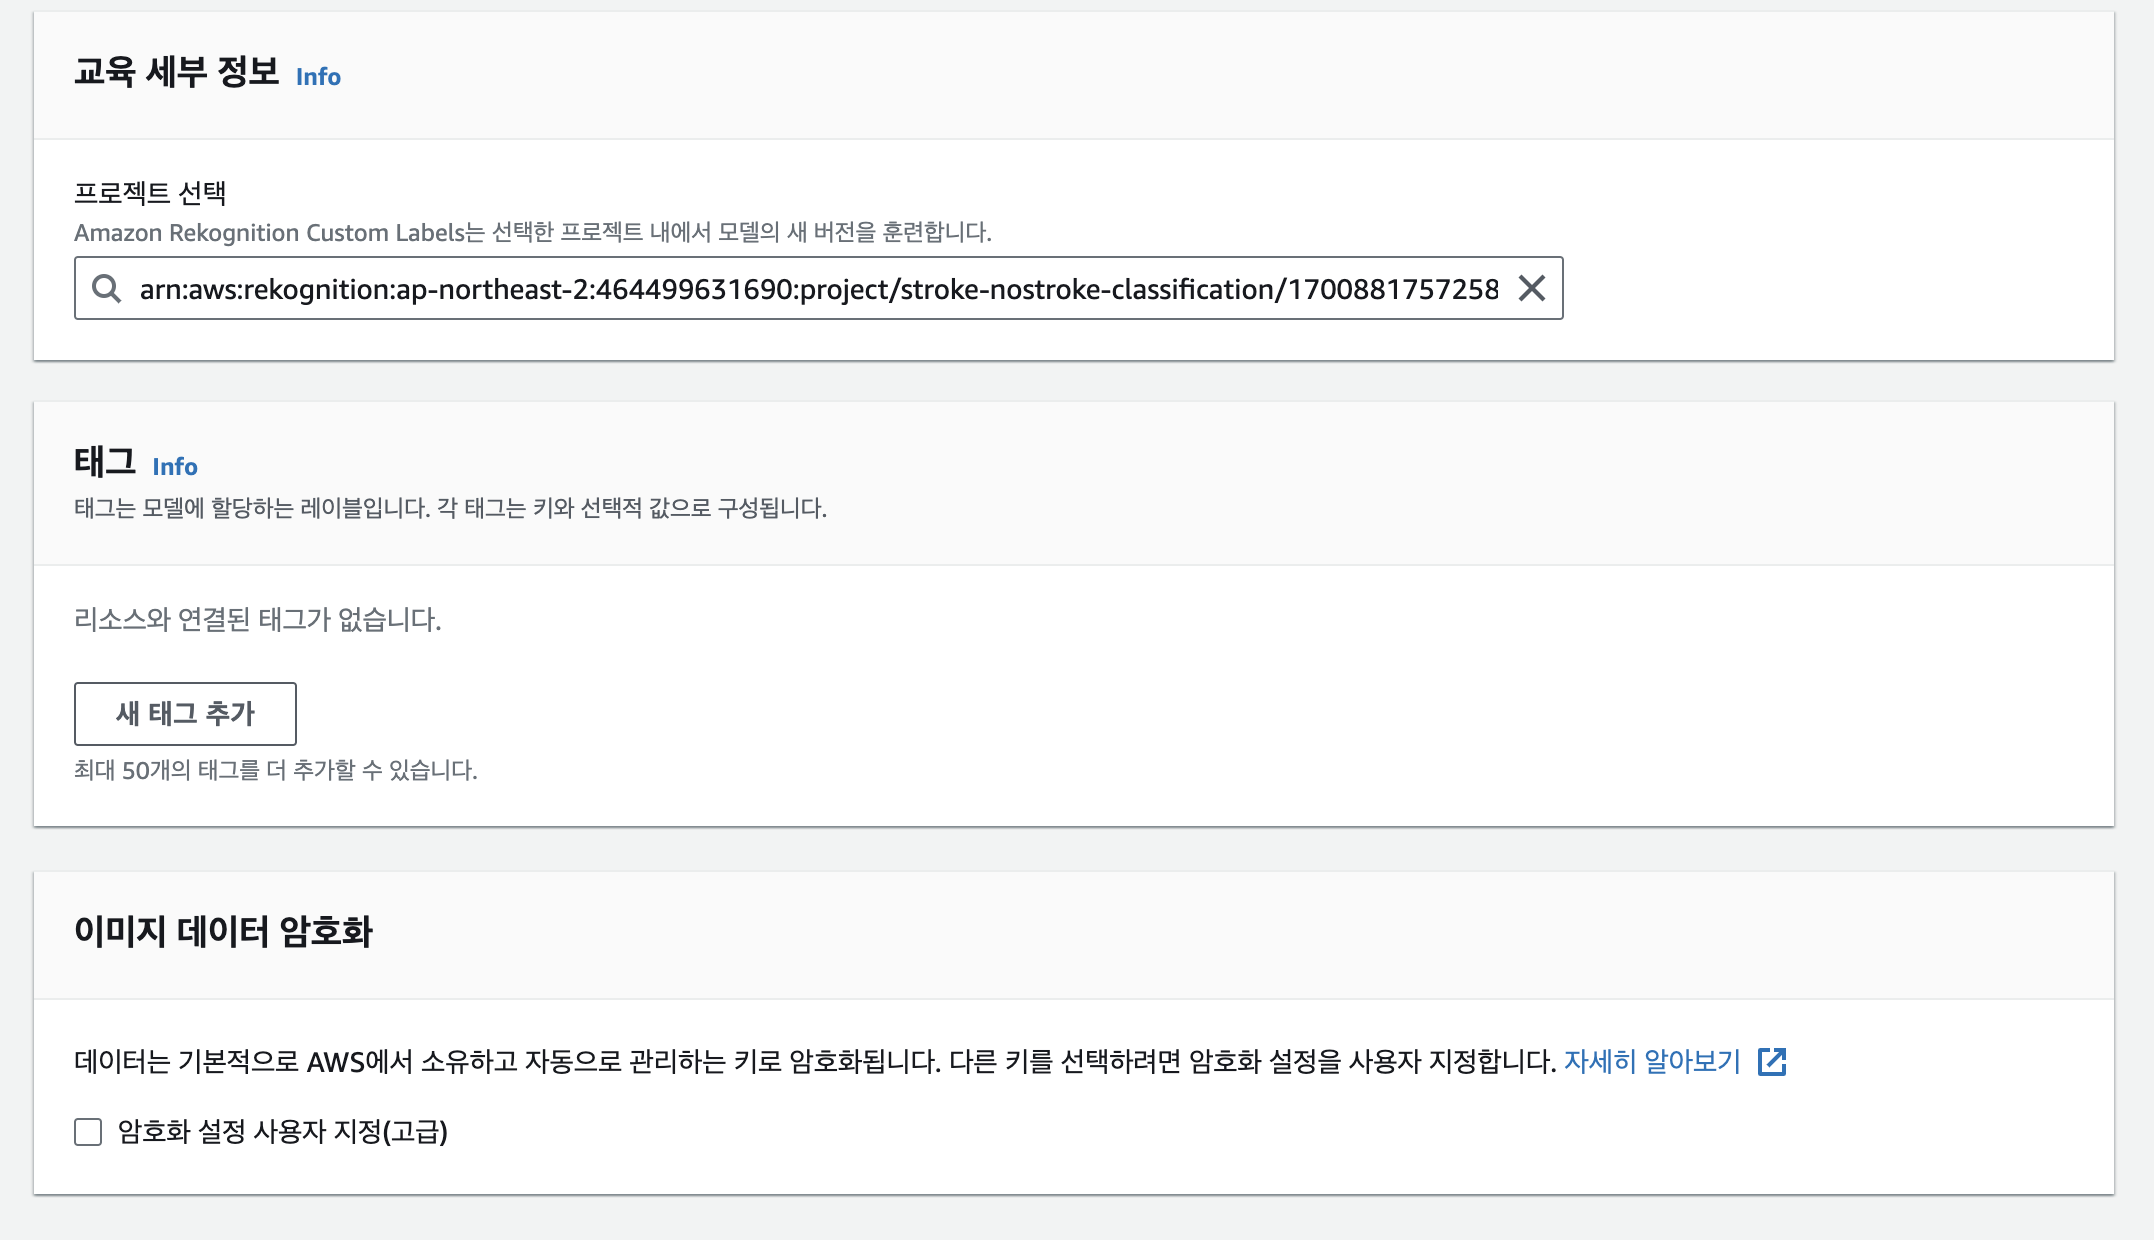
\includegraphics[width=8.5cm]{images/rek_training.png}
    \caption{Training Amazon Rekognition, Full automatic}
\end{figure}

\subsubsection{\textbf{Testing and Deploying trained model}}
% 모델의 학습이 종료되면 배포할 수 있다. 이로써 외부에서 학습된 모델에 접근할 수 있고, 따로 웹 서버를 만들고 실행할 필요 없다. 배포 전에 학습된 모델의 성능을 테스트한 결과도 볼 수 있다. 테스트 데이터 상에서 모든 결과를 정확하게 분류했다. 아래에서 볼 수 있듯이 F1 score 가 1이 나왔다. 그리고 각 데이터의 Confidence level도 상당히 높은 것으로 보아 모델의 학습이 매우 잘 이루어졌단 것을 알 수 있었다.
Once training of the model is complete, it can be distributed. This allows access to externally trained models, and there is no need to create and run a separate web server. You can also see the results of testing the performance of the learned model before deployment. All results were accurately classified on the test data. As you can see below, the F1 score was 1. Also, the confidence level of each data was quite high, showing that the model was trained very well.


\begin{figure}[h]
    \centering
    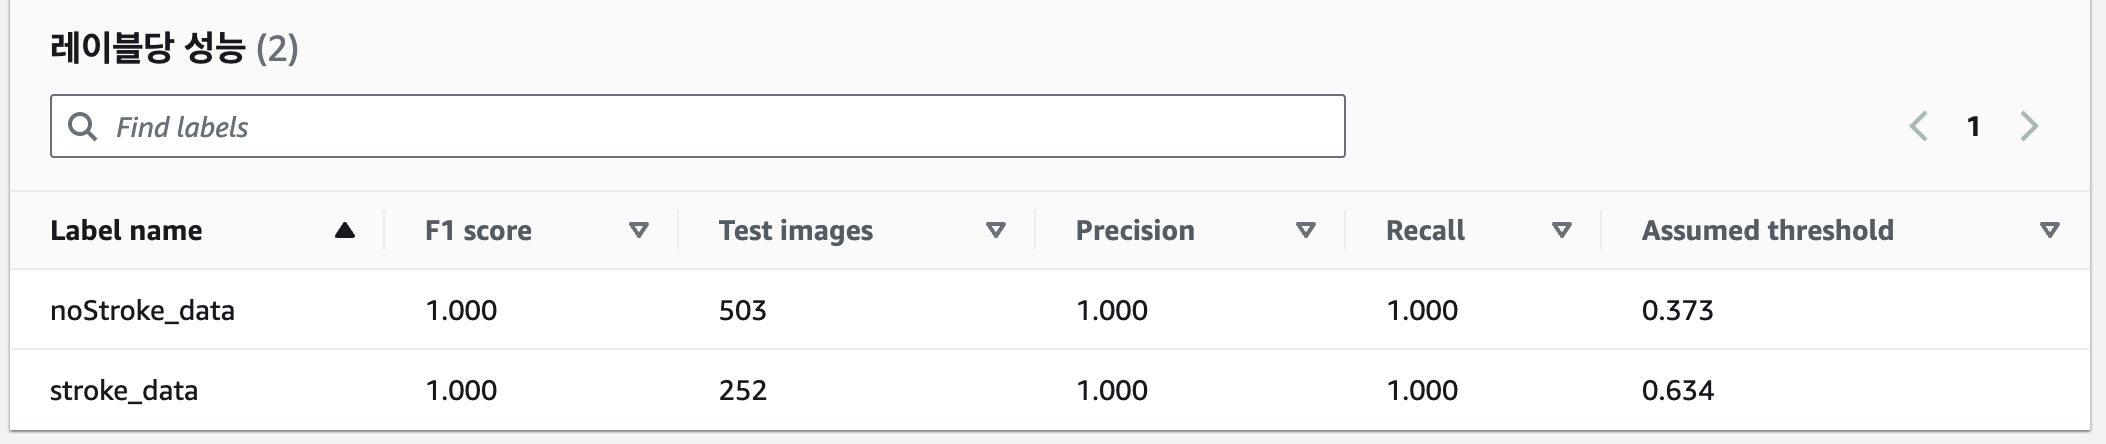
\includegraphics[width=8.5cm]{images/rek_result.png}
    \caption{Result of testing trained Rekogniton model}
\end{figure}


\begin{figure}[h]
    \centering
    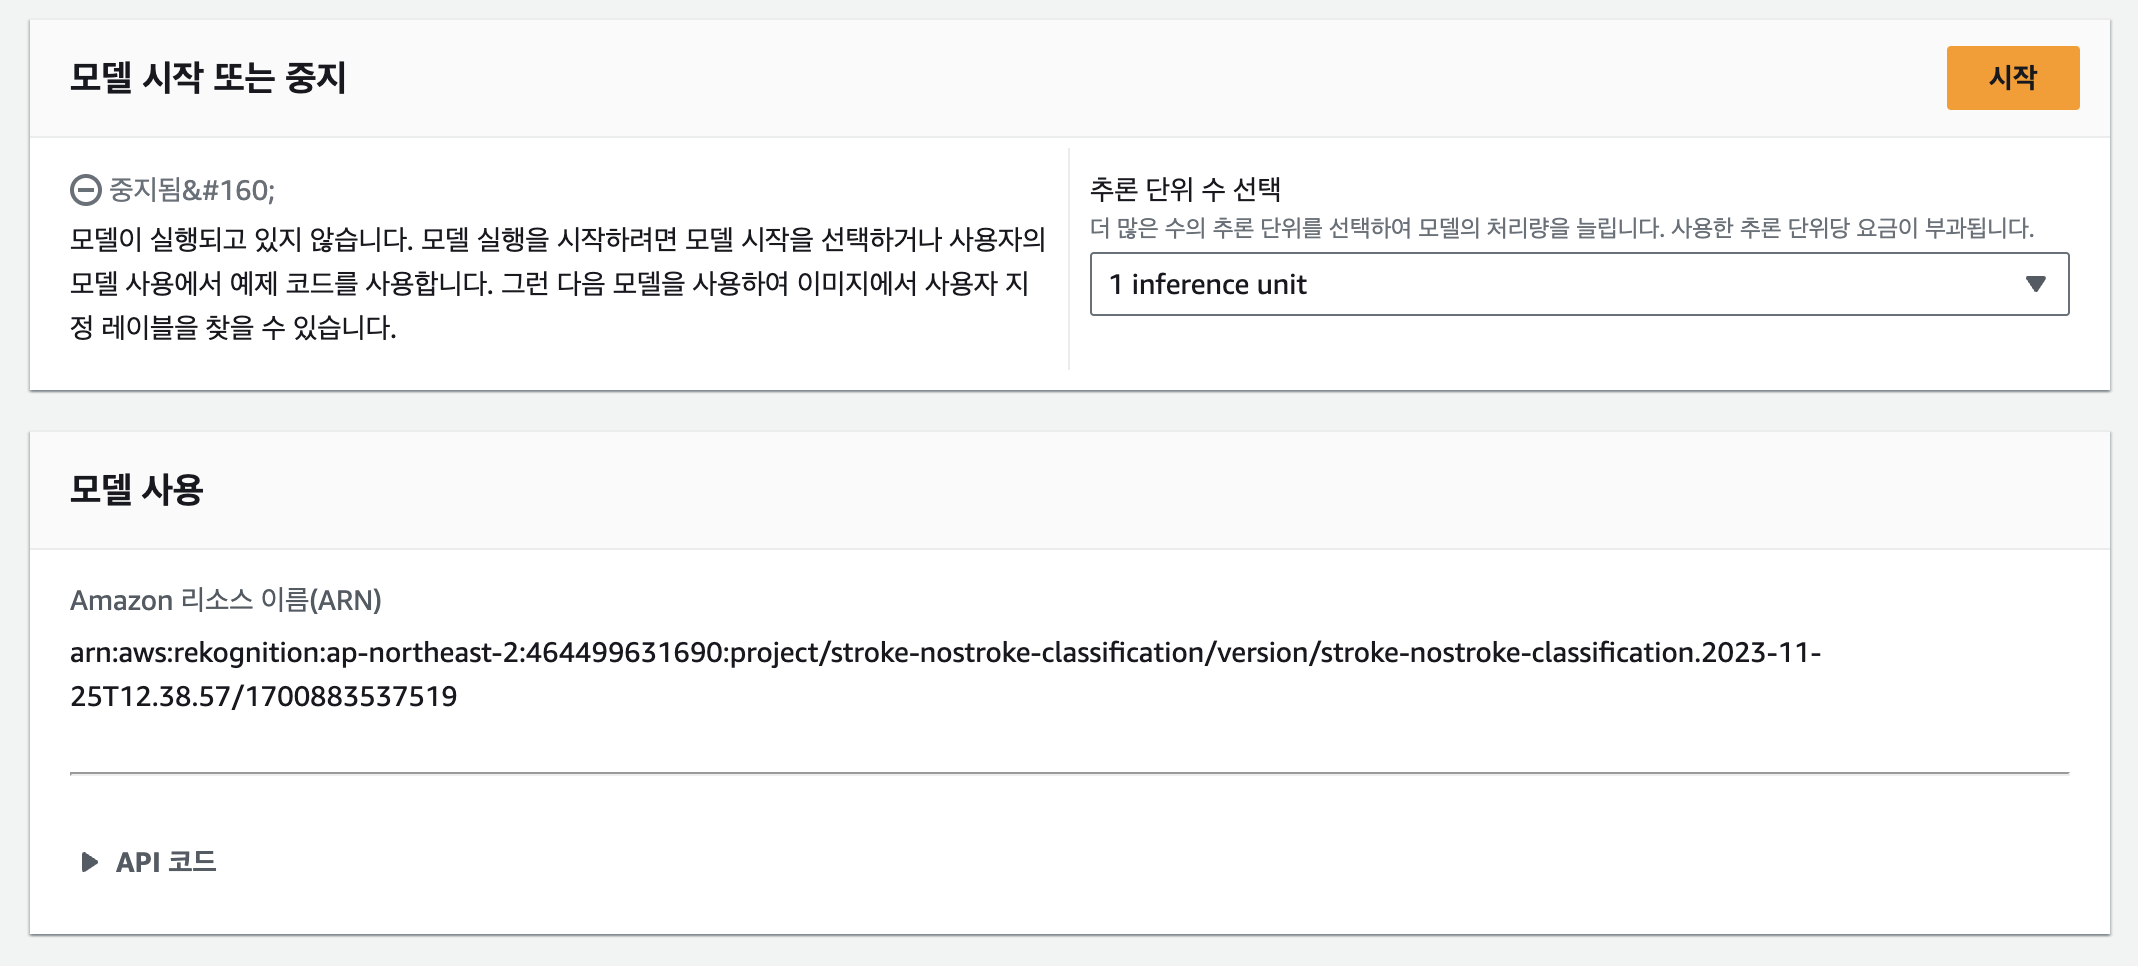
\includegraphics[width=8.5cm]{images/rek_deploy.png}
    \caption{Deploying trained Rekognition model}
\end{figure}


\subsection{\textbf{Raspberry Pi}}
\\

\subsubsection{\textbf{Raspberry OS installation and connection}}
To download the Raspberry Pi OS image, you will need a micro SD card. Recently, with the introduction of the Raspberry Pi Imager, downloading and installing the OS has become more convenient.
First, download the Raspberry Pi Imager on your local desktop. Then, insert the micro SD card into your desktop. In the Raspberry Pi Imager, select the SD card from the Storage tab and install the Raspberry Pi OS.
After that, insert the SD card into the Raspberry Pi, and connect the power using a USB-C port. Your Raspberry Pi will power on.\\

\subsubsection{\textbf{Wi-fi}}
\begin{figure}[h]
    \centering
    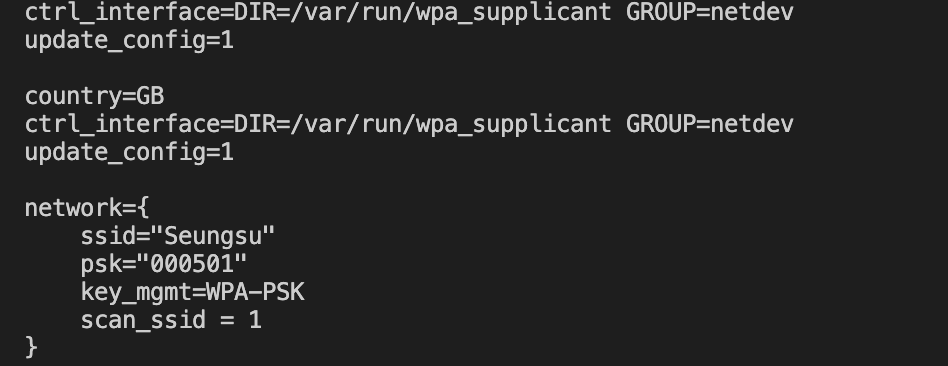
\includegraphics[width=0.5\linewidth]{images/wifi.png}
    \caption{Wifi Setting}
    \label{fig:enter-label}
\end{figure}
While Raspberry Pi does have a built-in Wi-Fi module, it doesn't automatically connect during boot. To enable this functionality, you need to modify the 'wpa\_supplicant.conf' file. Insert your Wi-Fi ID and password as shown below, and use 'scan\_ssid = 1' to allow detection of hidden networks. By making these changes to the 'wpa\_supplicant.conf' file, Raspberry Pi will automatically connect to Wi-Fi during boot. Wi-Fi connection is crucial not only for internet access but also for SSH usage.\\

\subsubsection{\textbf{SSH}}
\begin{figure}[h]
    \centering
    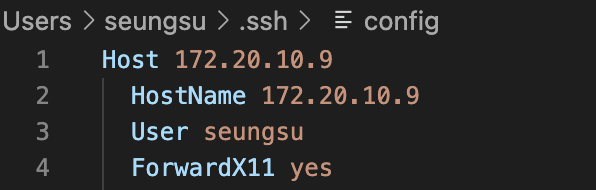
\includegraphics[width=0.5\linewidth]{images/ssh.png}
    \caption{SSH Setting}
    \label{fig:enter-label}
\end{figure}
You can configure SSH in the Raspberry Pi settings. Enabling SSH automatically completes the necessary settings. After that, when you first establish an SSH connection, set the connection password, and you are ready to use SSH.
\\

SSH primarily relies on IP for forwarding, so you need to know the current IP address of the Raspberry Pi, which you can check by entering 'ifconfig' in the terminal. Additionally, the local and remote devices you want to connect must be connected to the same Wi-Fi network by default.
After connecting your local desktop to the same Wi-Fi network as the Raspberry Pi, you can complete the SSH connection by entering 'ssh userID@xxx.xx.xx.x,' providing your username and IP address, and entering the password.\\

\subsubsection{\textbf{Camera}}
\begin{figure}[h]
    \centering
    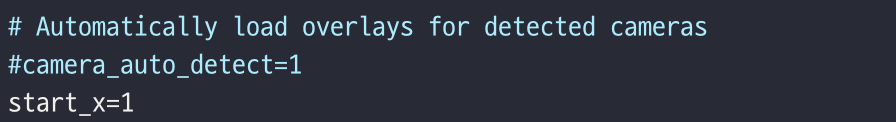
\includegraphics[width=0.5\linewidth]{images/camera.png}
    \caption{Camera Setting}
    \label{fig:enter-label}
\end{figure}
With the update of the Raspberry Pi OS to 'Bookworm,' there have been changes in the overall software for using the camera. The update involved transitioning to the 'libcamera' library, which posed challenges when applying it to essential camera functions, such as 'VideoCapture' in OpenCV. Therefore, it is necessary to revert to the previous version.

In the 'config.txt' file, you should provide the 'start\_x=1' parameter and turn off the 'camera\_auto\_detect' feature.\\

\subsubsection{\textbf{Virtual Environment for Python}}
Raspberry Pi is an externally managed environment, and as such, it restricts the use of 'pip,' allowing only 'apt' for package management. However, creating a Python virtual environment can provide more flexibility within these constraints. A significant reason for using Python is the availability of a wide range of libraries. To conveniently install these libraries, it is advisable to create a virtual environment.\\

\subsubsection{\textbf{Swap size}}
OpenCV is a sizable library, and to ensure stable operation, it's important to allocate sufficient disk space. You can determine the current swap size in use by using 'free -m.' Then, you can adjust the swap size by modifying '/etc/dphys-swapfile.' The default setting is 100, but to ensure normal operation, it's recommended to set it to 4096 or higher. After adjusting the swap size, you can proceed with the installation of OpenCV\\

\subsection{\textbf{OpenCV}}
\subsubsection{\textbf{video\_capture}}
 to use the 'VideoCapture' function properly, you need to downgrade the camera library and disable 'camera\_auto\_detect' to use OpenCV/V4L2. Additionally, increasing the GPU memory on the Raspberry Pi is recommended for improved video processing.\\

 \subsubsection{\textbf{Color scale converting}}
Using 'cv2.cvtColor,' the image being captured is converted to grayscale. This is used for the following reasons:\\

\begin{itemize}
\item Information Compression: Grayscale images have only one color channel per pixel, representing only brightness information. This reduces image size, saving memory and reducing computational requirements for storage and processing.\\
\item Computational Efficiency: Grayscale image processing is much faster and more efficient compared to color image processing. Handling a single color channel is faster and more efficient than multiple color channels.\\
\item Feature Extraction and Object Detection: Grayscale images are primarily used in image processing tasks such as edge detection, feature extraction, and object detection. Edge detection algorithms often rely on brightness information, making grayscale images more suitable for these tasks.\\
\item Memory Savings: Grayscale images require less memory compared to color images, which can be advantageous for memory-intensive tasks, such as deep learning models.\\
\end{itemize}

Facial recognition is possible with grayscale images, so changing to grayscale helps increase computational efficiency.\\

\subsection{\textbf{Amazone Polly}}
\subsubsection{AWS Account and IAM User Setup:}
Log in to the AWS Management Console.
Create an IAM user with the necessary permissions to use the Polly service. Assign the user the appropriate policies to allow Polly API calls.
\subsubsection{Install Boto3 Library:}
Install the boto3 library for Python, which is required for interacting with AWS services.
\subsubsection{Play the speach file:}
Depending on our device, Raspberry pi, We can use tools like pygame or cvlc to play the generated MP3 file.



\subsection{\textbf{Privacy Policy}}
To ensure personal data protection, we implement a two-step process:\\

\begin{enumerate}
    \item The first step involves blurring the background screen.
    \begin{enumerate}
    \item Backgroung Blur\\
    \end{enumerate}
    
    \item The second step uses a computer vision model that operates exclusively on the local device for initial assessment. Only if detection is made, the connection to the server is established. we called it 'Two-level detection'.
And if connected to the internet, an LED module lights up next to the camera, allowing customers to visually confirm whether the camera is online or not.\\
\\
    \textbf{Two-level detection:}
    \cite{gradient} Through the following research paper, we obtained the gradient difference at the corner of the mouth for stroke diagnosis using face detection. Utilizing the coordinates of each landmark obtained above, we issue a warning when the gradient exceeds a certain threshold.\\
    
    \begin{enumerate}
    \item \textbf{When No Detection Occurs in Fisrt-level:}\\
\\In the absence of detection in real-time, the system continues to operate actively within the user's daily life without any specific signals.\\
\item \textbf{When Detection Occurs in First-level:}\\
\\Upon detecting risk factors in real-time, the system establishes a connection to the server and captures a more accurate photo for further detection using a trained artificial intelligence model (e.g., SVM, Transformer), ensuring higher accuracy.\\
\item \textbf{When the Diagnosis indicates a Stroke in Second-level:}\\
\\In the event of a stroke diagnosis, the user is promptly informed.
After the notification, the system seeks the user's consent, and upon receiving it, automatically initiates a 119 emergency call.\\
\item \textbf{When the Diagnosis Indicates No Stroke:}\\
\\If no detection occurs in the initial assessment, the system continues its operation. However, in the secondary assessment, if no detection takes place, the user is informed to provide reassurance.

    \end{enumerate}
\end{enumerate}